% slides.tex
\documentclass[20pt]{beamer}
\usepackage{listings}
\usepackage[utf8]{inputenc}
\usepackage{color}
\usepackage{graphicx}

\usetheme{default}
\usecolortheme{dove}
\useoutertheme{default}

% Slightly smaller title
\setbeamerfont{frametitle}{size=\large}
\setbeamerfont{verb}{size=\small}

% lst settings
\lstset{
    language=Haskell,
    basicstyle=\small,
    gobble=4
}

\newcommand{\vspaced}{
    \vspace{5mm}
}

\begin{document}

\title{Digestive Functors 0.3}
\subtitle{GhentFPG}
\author{Jasper Van der Jeugt}
\date{March 20, 2012}

\begin{frame}[plain]
    \titlepage
\end{frame}

% Introduction
% ------------

\begin{frame}{Hello!}
    My name is Jasper \\
    Student at UGent \\
    I write Haskell \\
    GhentFPG \\
    \texttt{@jaspervdj} \\
    \texttt{jaspervdj.be}
    \begin{picture}(0.0, 0.0)
    \put(40.0, -15.0){
        
\includegraphics[width=0.5\textwidth]{../2011-functionalpx-blaze-html/images/hat.pdf}}
    \end{picture}
\end{frame}

% What are formlets?
% ------------------

\begin{frame}{Overview}
    \textbf{What are formlets?} \\
    digestive-functors \\
    digestive-functors 0.3 \\
\end{frame}

\begin{frame}{What are formlets?}
    Coined in a 2008 paper \\
    \vspaced
    \emph{The essence of form abstraction} \\
    \vspaced
    Ezra Cooper, Sam Lindley, Philip Wadler, and Jeremy Yallop. \\
    \vspaced
    Haskell library by Chris Eidhof
\end{frame}

\begin{frame}{What are formlets?}
    Idea: forms written using an \emph{Applicative Functor} approach are
    \emph{inherently composable}.
\end{frame}

\begin{frame}[fragile]{What are formlets?}
    \begin{lstlisting}
    data Date = Date
        { month :: Integer
        , day   :: Integer
        } deriving (Show)
    \end{lstlisting}
\end{frame}

\begin{frame}[fragile]{What are formlets?}
    \begin{lstlisting}
    validDate :: Date -> Bool
    validDate (Date m d) =
        m `elem` [1 .. 12] &&
        d `elem` [1 .. 31]
    \end{lstlisting}
\end{frame}

\begin{frame}[fragile]{What are formlets?}
    \begin{lstlisting}
    dateForm' :: Form Date
    dateForm' = Date
        <$> inputIntegerF (Just 1)
        <*> inputIntegerF (Just 16)
    \end{lstlisting}
    \begin{lstlisting}
    dateForm :: Form Date
    dateForm = dateForm' `check`
        ensure validDate
        "This is not a valid date"
    \end{lstlisting}
\end{frame}

\begin{frame}[fragile]{What are formlets?}
    \textbf{Composability?} \\
    \vspaced
    \begin{lstlisting}
    dateForm :: Form Date

    inputIntegerF (Just 1)
        :: Form Integer
    \end{lstlisting}
\end{frame}

\begin{frame}[fragile]{What are formlets?}
    \begin{lstlisting}
    data User = User
        { name      :: String
        , password  :: String
        , birthdate :: Date
        } deriving (Show)
    \end{lstlisting}
\end{frame}

\begin{frame}[fragile]{What are formlets?}
    \begin{lstlisting}
    userForm :: Form User
    userForm = User
        <$> inputF Nothing
        <*> passwordF Nothing
        <*> dateForm
    \end{lstlisting}
\end{frame}

% digestive-functors
% ------------------

\begin{frame}{Overview}
    What are formlets? \\
    \textbf{digestive-functors} \\
    digestive-functors 0.3 \\
\end{frame}

\begin{frame}{digestive-functors}
    Released in 2010 \\
    \vspaced
    A number of practical improvements in comparison to formlets \\
    \vspaced
    Similar API, completely different internals
\end{frame}

\begin{frame}[fragile]{digestive-functors}
    Allow user to click label instead of (small) checkbox \\
    \begin{lstlisting}[language=html]
    <label for="checkbox">
        Label:
    </label>
    <input type="checkbox"
        id ="checkbox" />
    \end{lstlisting}
\end{frame}

\begin{frame}[fragile]{digestive-functors}
    Error type in formlets:
    \begin{lstlisting}
    [String]
    \end{lstlisting}
    \vspaced
    Error type in digestive-functors:
    \begin{lstlisting}
    [ErrorDescription] -> Html
    \end{lstlisting}
\end{frame}

\begin{frame}{digestive-functors}
    In formlets:
    \vspaced
    \begin{center}
    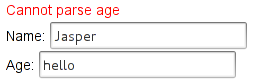
\includegraphics[width=0.7\textwidth]{images/errors-formlets.png}
    \end{center}
\end{frame}

\begin{frame}{digestive-functors}
    In digestive-functors:
    \vspaced
    \begin{center}
    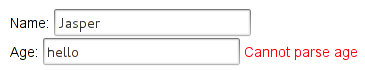
\includegraphics[width=\textwidth]{images/errors-digestive-functors.png}
    \end{center}
\end{frame}

\begin{frame}{digestive-functors}
    \textbf{Problems:} \\
    \vspaced
    Sometimes hard to use \\
    Suffered from TMTVA* Syndrome \\
    Complicated implementation \\
    \vspaced
    \emph{*Too Many Type Variables, Aaargh!}
\end{frame}

% digestive-functors 0.3
% ----------------------

\begin{frame}{Overview}
    What are formlets? \\
    digestive-functors \\
    \textbf{digestive-functors 0.3} \\
\end{frame}

\begin{frame}{digestive-functors 0.3}
    What I've been working on for some weeks \\
    \vspaced
    Attempts to overcome the main drawback of formlets
\end{frame}

\begin{frame}[fragile]{digestive-functors 0.3}
    \begin{lstlisting}
    foo :: Form User
    \end{lstlisting}
    \vspaced
    Specifies the \emph{validation rules} as well as the \emph{HTML layout}
\end{frame}

\begin{frame}{digestive-functors 0.3}
    \textbf{Separation of concerns}
    \vspaced
    \begin{itemize}
    \item Create multiple representations for a single form
    \item Cleaner validation rules code
    \item Use different HTML templating engines
    \end{itemize}
\end{frame}

\begin{frame}{digestive-functors 0.3}
    \textbf{Disadvantage: some loss of type-safety} \\
    \vspaced
    Probably impossible to have a type-safe coupling of view and validation
    rules without losing flexibility or ease-of-use \\
    \vspaced
    Explanation does not fit on this slide \\
\end{frame}

\begin{frame}[fragile]{digestive-functors 0.3}
    \begin{lstlisting}
    dateForm' :: Form Date
    dateForm' = Date
        <$> "month" .: stringRead'
        <*> "day"   .: stringRead'
      where
        stringRead' = stringRead
            "Can't parse"
    \end{lstlisting}
\end{frame}

\begin{frame}[fragile]{digestive-functors 0.3}
    \begin{lstlisting}
    dateForm :: Form Date
    dateForm = check
        "This is not a valid date"
        validDate
        dateForm'
    \end{lstlisting}
\end{frame}

\begin{frame}[fragile]{digestive-functors 0.3}
    \begin{lstlisting}
    dateView view = do
        errorList "month" view
        label "month" view "Name: "
        inputText "month" view
        H.br

        errorList "day" view
        label "day" view "Email: "
        inputText "day" view
        H.br
    \end{lstlisting}
\end{frame}

\begin{frame}[fragile]{digestive-functors 0.3}
    \textbf{Composability} \\
    \vspaced
    \begin{lstlisting}
    userForm :: Form User
    userForm = User
        <$> "name"      .: string'
        -- Password is just a string!
        <*> "password"  .: string'
        <*> "birthdate" .: dateForm
      where
        string' = string Nothing
    \end{lstlisting}
\end{frame}

\begin{frame}[fragile]{digestive-functors 0.3}
    \begin{lstlisting}
    userView :: View Html -> Html
    userView view = do
        label "name" view "Name: "
        inputText "name" view
        H.br

        label "name" view "Name: "
        inputPassword "name" view
        H.br
        ...
    \end{lstlisting}
\end{frame}

\begin{frame}[fragile]{digestive-functors 0.3}
    \begin{lstlisting}
    userView :: View Html -> Html
    userView view = do
        ...
        label "birthdate.month"
            view "Month: "
        inputText "birthdate.month"
            view
        H.br
    \end{lstlisting}
\end{frame}

\begin{frame}[fragile]{digestive-functors 0.3}
    \begin{lstlisting}
    userView :: View Html -> Html
    userView view = do
        ...
        dateView $
            subView "birthdate" view
    \end{lstlisting}
\end{frame}

\begin{frame}[plain]
    \begin{center}
    \huge{Demo}
    \end{center}
\end{frame}

\end{document}
